\documentclass{standalone}
\usepackage{tikz}
\usetikzlibrary{arrows.meta, positioning, backgrounds, fit}
\usepackage{xcolor}
\colorlet{myred}{green!60!black}
\colorlet{myblue}{red!80!black}
\colorlet{mybluee}{myblue!80!black}
\colorlet{mygreen}{blue!80!black}
\colorlet{myorange}{orange!70!red!60!black}
\colorlet{mydarkred}{red!30!black}
\colorlet{mydarkblue}{blue!40!black}
\colorlet{mydarkgreen}{green!30!black}
\begin{document}
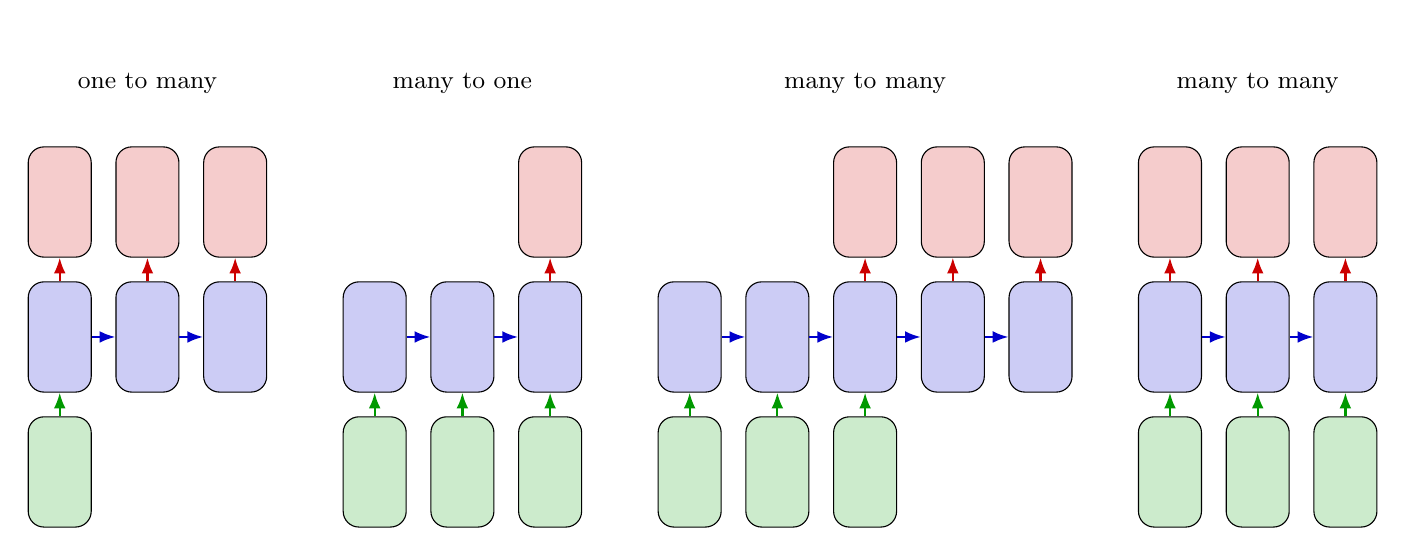
\begin{tikzpicture}[
    node distance=0.3cm and 0.3cm,
    every node/.style={minimum width=0.8cm, minimum height=1.4cm, align=center, draw=none, rounded corners=0.2cm},
    arrow/.style={-{Latex[length=2mm]}, thick}
]
% One to Many
\begin{scope}[local bounding box=diagram1]
    \node[fill=myblue!20, draw] (o11) {};
    \node[fill=myblue!20, draw, right=of o11] (o12) {};
    \node[fill=myblue!20, draw, right=of o12] (o13) {};
    \node[fill=mygreen!20, draw, below=of o11] (h11) {};
    \node[fill=mygreen!20, draw, right=of h11] (h12) {};
    \node[fill=mygreen!20, draw, right=of h12] (h13) {};
    \node[fill=myred!20, draw, below=of h11] (i11) {};
    \foreach \i/\j in {h11/o11, h12/o12, h13/o13} {
        \draw[arrow, myblue] (\i) -- (\j);
    }
    \foreach \i/\j in {i11/h11} {
        \draw[arrow, myred] (\i) -- (\j);
    }
    \foreach \i/\j in {h11/h12, h12/h13} {
        \draw[arrow, mygreen] (\i) -- (\j);
    }
\end{scope}
\node[draw=none, above=0.1cm of o12, font=\small] {one to many};

% Many to One
\begin{scope}[local bounding box=diagram2, xshift=4cm]
    \node[fill=white!20] (o21) {};
    \node[fill=white!20, right=of o21] (o22) {};
    \node[fill=myblue!20, draw, right=of o22] (o23) {};
    \node[fill=mygreen!20, draw, below=of o21] (h21) {};
    \node[fill=mygreen!20, draw, right=of h21] (h22) {};
    \node[fill=mygreen!20, draw, right=of h22] (h23) {};
    \node[fill=myred!20, draw, below=of h21] (i21) {};
    \node[fill=myred!20, draw, below=of h22] (i22) {};
    \node[fill=myred!20, draw, below=of h23] (i23) {};
    \foreach \i/\j in {h23/o23} {
        \draw[arrow, myblue] (\i) -- (\j);
    }
    \foreach \i/\j in {i21/h21, i22/h22, i23/h23} {
        \draw[arrow, myred] (\i) -- (\j);
    }
    \foreach \i/\j in {h21/h22, h22/h23} {
        \draw[arrow, mygreen] (\i) -- (\j);
    }
\end{scope}
\node[draw=none, above=0.1cm of o22, font=\small] {many to one};

% Many to Many (first version)
\begin{scope}[local bounding box=diagram3, xshift=8cm]
    \node[fill=white!20] (o31) {};
    \node[fill=white!20, right=of o31] (o32) {};
    \node[fill=myblue!20, draw, right=of o32] (o33) {};
    \node[fill=myblue!20, draw, right=of o33] (o34) {};
    \node[fill=myblue!20, draw, right=of o34] (o35) {};
    \node[fill=mygreen!20, draw, below=of o31] (h31) {};
    \node[fill=mygreen!20, draw, right=of h31] (h32) {};
    \node[fill=mygreen!20, draw, right=of h32] (h33) {};
    \node[fill=mygreen!20, draw, right=of h33] (h34) {};
    \node[fill=mygreen!20, draw, right=of h34] (h35) {};
    \node[fill=myred!20, draw, below=of h31] (i31) {};
    \node[fill=myred!20, draw, below=of h32] (i32) {};
    \node[fill=myred!20, draw, below=of h33] (i33) {};
    \foreach \i/\j in {h33/o33, h34/o34, h35/o35} {
        \draw[arrow, myblue] (\i) -- (\j);
    }
    \foreach \i/\j in {i31/h31, i32/h32, i33/h33} {
        \draw[arrow, myred] (\i) -- (\j);
    }
    \foreach \i/\j in {h31/h32, h32/h33, h33/h34, h34/h35} {
        \draw[arrow, mygreen] (\i) -- (\j);
    }
\end{scope}
\node[draw=none, above=0.1cm of o33, font=\small] {many to many};

% Many to Many (second version)
\begin{scope}[local bounding box=diagram4, xshift=14.1cm]
    \node[fill=myblue!20, draw] (o41) {};
    \node[fill=myblue!20, draw, right=of o41] (o42) {};
    \node[fill=myblue!20, draw, right=of o42] (o43) {};
    \node[fill=mygreen!20, draw, below=of o41] (h41) {};
    \node[fill=mygreen!20, draw, right=of h41] (h42) {};
    \node[fill=mygreen!20, draw, right=of h42] (h43) {};
    \node[fill=myred!20, draw, below=of h41] (i41) {};
    \node[fill=myred!20, draw, below=of h42] (i42) {};
    \node[fill=myred!20, draw, below=of h43] (i43) {};
    \foreach \i/\j in {h41/o41, h42/o42, h43/o43} {
        \draw[arrow, myblue] (\i) -- (\j);
    }
    \foreach \i/\j in {i41/h41, i42/h42, i43/h43} {
        \draw[arrow, myred] (\i) -- (\j);
    }
    \foreach \i/\j in {h41/h42, h42/h43} {
        \draw[arrow, mygreen] (\i) -- (\j);
    }
\end{scope}
\node[draw=none, above=0.1cm of o42, font=\small] {many to many};

\end{tikzpicture}
\end{document}